\originalchapter{8.323 作业12题解}
题源:MIT OCW,8.323,2023年春季,2023年5月2日发布;本学期最后一套,90分加30分奖励.\href{https://ocw.mit.edu/courses/8-323-relativistic-quantum-field-theory-i-spring-2023/mit8_323_s23_pset12.pdf}{原作业PDF};\href{https://ocw.mit.edu/courses/8-323-relativistic-quantum-field-theory-i-spring-2023/mit8_323_s23_pset_12sol.pdf}{官方解PDF}.以下为官方解中文重编与独立补充,并非MIT官方中文版;MIT OCW来源,CC BY-NC-SA 4.0.原资料$(-+++)$已经换为$(+---)$,$s=(p_1+p_2)^2$、$t=(p_1-k_1)^2$、$u=(p_1-k_2)^2$,故$s+t+u$等于四条外腿质量平方之和.

统一使用$S_{fi}=\delta_{fi}+\ii(2\pi)^4\delta^{(4)}(P_f-P_i)\mathcal M_{fi}$及Lorentz不变相空间
\[
 \dd\Phi_n=(2\pi)^4\delta^{(4)}(P_i-\textstyle\sum_jk_j)
 \prod_j\frac{\dd^3k_j}{(2\pi)^3 2E_j}.
\]
源资料的$M$有时指完整图的$\ii\mathcal M$;模方相同.衰变和散射分别满足\[\dd\Gamma=\frac{|\mathcal M|^2}{2E_i}\dd\Phi_n,\qquad\dd\sigma=\frac{|\mathcal M|^2}{4\sqrt{(p_1\cdot p_2)^2-m_1^2m_2^2}}\dd\Phi_n.\]若对全动量域积分,相同末态的每组$m$个粒子再除$m!$.两体质心系有
\[
 \frac{\dd\sigma_{\rm labelled}}{\dd\Omega}=\frac{|\mathcal M|^2}{64\pi^2s}\frac{|\mathbf k|}{|\mathbf p|},
\]
这里“labelled”表示两末态动量按$k_1,k_2$标记;相同粒子的物理事件可取半个角域,或全角域时加$1/2$.

\originalsection{原题1}
\begin{exercise}
考虑两个实标量场
\[
 \Lag=\frac12(\partial\phi)^2-\frac12M^2\phi^2
 +\frac12(\partial\chi)^2-\frac12m^2\chi^2+\frac g2\phi\chi^2.
\]
假设$M>2m$且$g$很小,求$\phi$粒子最低阶衰变率.
\end{exercise}
\begin{solution}
相互作用的$1/2$抵消两条相同$\chi$外腿的收缩数,顶点为$\ii g$,故$\mathcal M=g$.只有如下树图:
\begin{center}\begin{tikzpicture}[scale=.8]
\draw[dashed](-2,0)node[left]{$\phi$}--(0,0);\draw(0,0)--(1.5,1)node[right]{$\chi(k_1)$};\draw(0,0)--(1.5,-1)node[right]{$\chi(k_2)$};
\end{tikzpicture}\end{center}
在$\phi$静止系,先用空间delta置$\mathbf k_2=-\mathbf k_1$,再用$\delta(M-2E_k)$求径向积分:
\begin{align*}
 \dd\Phi_2&=\frac1{(2\pi)^2}\frac{k^2\dd k}{4E_k^2}\delta(M-2E_k)\dd\Omega\\
 &=\frac{k_*}{32\pi^2E_*}\dd\Omega
 =\frac1{32\pi^2}\sqrt{1-\frac{4m^2}{M^2}}\dd\Omega,
 \quad E_*=\frac M2,\quad k_*=\sqrt{M^2/4-m^2}.
\end{align*}
用$\dd E_k/\dd k=k/E_k$可核对delta的Jacobian.对全立体角积分并除相同粒子$2!$:
\[
 \Gamma_{\rm rest}=\frac1{2M}\frac1{2!}g^2\frac1{8\pi}
 \sqrt{1-\frac{4m^2}{M^2}}
 =\frac{g^2}{32\pi M}\sqrt{1-\frac{4m^2}{M^2}}.
\]
这是振幅$\order(g)$导致的$\order(g^2)$宽度.运动系单位实验室时间的率为$\Gamma(E)=M\Gamma_{\rm rest}/E$;题目通常取本征寿命对应的静止宽度.
\end{solution}

\originalsection{原题2}
\begin{exercise}
用标量模型模拟$e^+e^-\to\gamma\to q\bar q$:电子与正电子的角色都由无质量实场$\psi$承担,无质量实场$\phi$模拟光子,有质量$m$的实场$\chi$模拟夸克.理论为
\[
 \Lag=\frac12(\partial\psi)^2+\frac12(\partial\phi)^2+\frac12(\partial\chi)^2
 -\frac12m^2\chi^2+\frac{g'}2\phi\psi^2+\frac g2\phi\chi^2,
\]
$g,g'$很小且阶数相当.(a) 求$\psi\psi\to\chi\chi$最低阶总截面,用$s,t,u$表示;(b) 求$\psi\psi\to\psi\psi$最低阶微分截面,用$s,t,u$表示.
\end{exercise}
\begin{solution}
(a) 外腿种类限制只允许一张$s$道图,$\psi\psi$在一个顶点汇合,内部$\phi$连接到$\chi\chi$顶点:
\begin{center}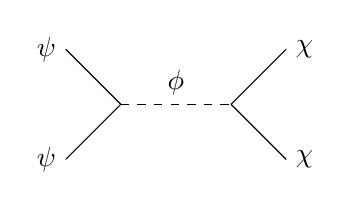
\begin{tikzpicture}[scale=.7]
\draw(-2,1)node[left]{$\psi$}--(-1,0);\draw(-2,-1)node[left]{$\psi$}--(-1,0);\draw[dashed](-1,0)--(1,0)node[midway,above]{$\phi$};\draw(1,0)--(2,1)node[right]{$\chi$};\draw(1,0)--(2,-1)node[right]{$\chi$};
\end{tikzpicture}\end{center}
两顶点$\ii g'$、$\ii g$及传播子$\ii/(s+\ii0)$给$\mathcal M=-gg'/(s+\ii0)$.质心能量$E=\sqrt s/2$,初态$|\mathbf p|=E$,末态$|\mathbf k|=\sqrt{E^2-m^2}$,所以
\[
 \frac{\dd\sigma_{\rm labelled}}{\dd\Omega}=\frac{g^2g'^2}{64\pi^2s^3}
 \sqrt{1-\frac{4m^2}{s}}.
\]
角度不依赖性源于交换粒子为标量且顶点无导数.对全角域积分再除$2!$得到
\[
 \sigma_{\rm tot}=\frac{g^2g'^2}{32\pi s^3}\sqrt{1-\frac{4m^2}{s}},\quad s\geq4m^2,
\]
阈值以下为零.$s+t+u=2m^2$,$t=m^2-s/2+(s/2)\sqrt{1-4m^2/s}\cos\theta$,$u$为最后一项反号,给出完整运动学域.

(b) 同一种$\psi$外腿允许$s,t,u$三个道:
\begin{center}\begin{tikzpicture}[scale=.65]
\draw(-2,1)--(-1,0);\draw(-2,-1)--(-1,0);\draw[dashed](-1,0)--(1,0);\draw(1,0)--(2,1);\draw(1,0)--(2,-1);\node at(0,-1.6){$s$};
\draw(4,1)--(6,1);\draw(4,-1)--(6,-1);\draw[dashed](5,1)--(5,-1);\node at(5,-1.6){$t$};
\draw(9,1.5)--(10,1);\draw(10,1)--(11,-1.5);\draw(9,-1.5)--(10,-1);\draw(10,-1)--(11,1.5);\draw[dashed](10,1)--(10,-1);\node at(10,-1.6){$u$(交换末腿)};
\end{tikzpicture}\end{center}
三个图相加而非相减,$\mathcal M=-g'^2(1/s+1/t+1/u)$(离开极点时省略$i0$).因此
\[
 \frac{\dd\sigma_{\rm labelled}}{\dd\Omega}=
 \frac{g'^4}{64\pi^2s}\left(\frac1s+\frac1t+\frac1u\right)^2.
\]
质量皆零时$s+t+u=0$,$t=-s(1-\cos\theta)/2$、$u=-s(1+\cos\theta)/2$,也可写
\[
 \frac{\dd\sigma_{\rm labelled}}{\dd\Omega}
 =\frac{g'^4}{64\pi^2s^3}\left(1-\frac4{\sin^2\theta}\right)^2,
 \qquad0<\theta<\pi.
\]
官方解把这题耦合写成$g$并漏掉角度式中的$s^{-2}$,这里按作用量与量纲纠正.全角域事件密度再除2;无角度截止的总截面在前后向极点发散,所以题目只要求微分截面,不存在这里的有限总截面答案.
\end{solution}

\originalsection{原题3}
\begin{exercise}
Rutherford散射:原作业(a)–(c)仅写“Peskin \& Schroeder: Prob. 4.4”,没有提供这三小问题面.本稿保留这一商业教材引用缺口,不从官方解反向重造教材题面,也不把解答PDF视为教材内容授权.

(d) 加分题:在相对论区域重复(c)的计算,对初态自旋平均、末态自旋求和,证明电子Coulomb散射截面为题面所示表达,其中$\alpha=e^2/(4\pi)$、$\mathbf p$为电子动量、$\beta$为速度.原PDF印为
\[
 \frac{\dd\sigma}{\dd\Omega}=\frac{\alpha^2}{4|\mathbf p|^2\beta^2\sin^2(\theta/2)}
 [1-\beta^2\sin^2(\theta/2)].
\]
这里分母$\sin^2$是原题排印错误;实际要证的Mott/Rutherford表达为$\sin^4$.本题可获的(d)按下列独立补充模型完成:电荷$Ze$的无限重静止点源产生$A^0=Ze/(4\pi r)$、$\mathbf A=0$,取Born最低阶;原目标式对应$Z=1$.
\end{exercise}
\begin{solution}
(a)–(c)没有公开题面,本稿不宣称完成这些教材子问.以下只完成可获(d),并明确补上它所依赖的外场模型假设.

静态势的单粒子Born振幅为$\mathcal M=-e\bar u(p')\gamma^\mu u(p)\widetilde A_\mu(\mathbf q)$,$\mathbf q=\mathbf p'-\mathbf p$.它由相互作用$-e\bar\psi\gamma^\mu\psi A_\mu$的一阶展开得出,时间积分给$2\pi\delta(E'-E)$;此处没有空间动量守恒delta,因为外场吸收动量.

为计算$1/r$的Fourier变换,先取$A^0_\mu(r)=Ze\e^{-\mu r}/(4\pi r)$,$\mu>0$.以$\mathbf q$为极轴,角积分给$2\sin(qr)/(qr)$,随后径向积分给
\[
 \widetilde A^0_\mu(\mathbf q)=\frac{Ze}{q^2+\mu^2},\qquad
 \widetilde A^0(\mathbf q)=\frac{Ze}{q^2}\quad(q\ne0).
\]
因此$\mathcal M=-Ze^2\bar u(p')\gamma^0u(p)/q^2$.定义$\overline{|\mathcal M|^2}$为$1/2$初态自旋平均与末态自旋和,则
\begin{align*}
 \overline{|\mathcal M|^2}
 &=\frac{Z^2e^4}{2q^4}\Tr[(\slashed p'+m)\gamma^0(\slashed p+m)\gamma^0]\\
 &=\frac{2Z^2e^4}{q^4}[2E^2-p'\cdot p+m^2]\\
 &=\frac{4Z^2e^4 E^2}{q^4}[1-\beta^2\sin^2(\theta/2)],
\end{align*}
用了$E'=E$、$|\mathbf p'|=p$、$p'\cdot p=E^2-p^2\cos\theta$以及$q^2=4p^2\sin^2(\theta/2)$;这里$q^2$指三维$|\mathbf q|^2$,不是四维$t$.

外场散射只有一个末态粒子,归一化和初态流给
\[
 \dd\sigma=\frac1\beta\frac1{2E}\frac{\dd^3p'}{(2\pi)^3 2E'}
 (2\pi)\delta(E'-E)\overline{|\mathcal M|^2}.
\]
用$\delta(E'-E)=(E/p)\delta(p'-p)$完成径向积分,$p/E=\beta$抵消入射流,故$\dd\sigma/\dd\Omega=\overline{|\mathcal M|^2}/(16\pi^2)$.代入上式得到
\[
 \boxed{\frac{\dd\sigma}{\dd\Omega}
 =\frac{Z^2\alpha^2}{4p^2\beta^2\sin^4(\theta/2)}
 [1-\beta^2\sin^2(\theta/2)]}.
\]
低速时$p\simeq m\beta$,括号趋于1,得到$Z^2\alpha^2/[4m^2\beta^4\sin^4(\theta/2)]$.前向$\theta=0$极点来自无限程点Coulomb势,不能在无屏蔽条件下积分为有限总截面.
\end{solution}

\originalsection{原题4}
\begin{exercise}
考虑$e^-+\mu^-\to e^-+\mu^-$,质量$m_e,m_\mu$.
(a) 求振幅;(b) 求$\frac14\sum_{\rm spin}|\mathcal M|^2$,即初态两粒子自旋平均、末态自旋求和,用$s,t,u$表示;(c) 加分题:求质心系微分截面;(d) 加分题:求muon静止实验室系的微分截面,并证明$m_\mu\to\infty$恢复原题3(d)的Rutherford/Mott公式.原题允许参考Peskin--Schroeder第5.4节,但要求自行完成中间计算.
\end{exercise}
\begin{solution}
(a) 记$p_1,p_2$为初态电子、muon,$k_1,k_2$为末态,$q=p_1-k_1=k_2-p_2$、$t=q^2$.最低阶只有一个光子$t$道;电子与muon不同,无交换外线图.
\begin{center}\begin{tikzpicture}[>=Stealth,scale=.9]
\draw[->](-2,1)node[left]{$e(p_1)$}--(0,1);\draw[->](0,1)--(2,1)node[right]{$e(k_1)$};
\draw[->](-2,-1)node[left]{$\mu(p_2)$}--(0,-1);\draw[->](0,-1)--(2,-1)node[right]{$\mu(k_2)$};
\draw[decorate,decoration={snake,amplitude=2pt,segment length=6pt}](0,-1)--(0,1)node[midway,right]{$\gamma$};
\end{tikzpicture}\end{center}
两个$-\ii e\gamma^\mu$顶点及Feynman规范传播子$-\ii\eta_{\mu\nu}/(t+\ii0)$给
\[
 \mathcal M=\frac{e^2}{t+\ii0}
 [\bar u_e(k_1)\gamma^\mu u_e(p_1)]
 [\bar u_\mu(k_2)\gamma_\mu u_\mu(p_2)].
\]
流守恒$q_\mu\bar u(k)\gamma^\mu u(p)=0$由两端同质量Dirac方程保证,故规范参数相关纵向传播项不贡献.

(b) 自旋和$\sum_su_s\bar u_s=\slashed p+m$将模方写成
\[
 \overline{|\mathcal M|^2}=\frac{e^4}{4t^2}
 \Tr[(\slashed k_1+m_e)\gamma^\mu(\slashed p_1+m_e)\gamma^\nu]
 \Tr[(\slashed k_2+m_\mu)\gamma_\mu(\slashed p_2+m_\mu)\gamma_\nu].
\]
四gamma迹为$4(\eta^{\alpha\mu}\eta^{\beta\nu}-\eta^{\alpha\beta}\eta^{\mu\nu}+\eta^{\alpha\nu}\eta^{\mu\beta})$,奇迹为零,故第一个迹为
$4[k_1^\mu p_1^\nu+k_1^\nu p_1^\mu-(k_1\cdot p_1-m_e^2)\eta^{\mu\nu}]$,第二个同理.将四项交叉收缩,得到
\begin{align*}
 \overline{|\mathcal M|^2}=\frac{8e^4}{t^2}\big[&
 (p_1\cdot p_2)(k_1\cdot k_2)+(p_1\cdot k_2)(k_1\cdot p_2)\\
 &-m_e^2(p_2\cdot k_2)-m_\mu^2(p_1\cdot k_1)+2m_e^2m_\mu^2\big].
\end{align*}
令$A=m_e^2+m_\mu^2$,各点积为
$p_1\cdot p_2=k_1\cdot k_2=(s-A)/2$,
$p_1\cdot k_2=k_1\cdot p_2=(A-u)/2$,
$p_1\cdot k_1=m_e^2-t/2$、$p_2\cdot k_2=m_\mu^2-t/2$.因此
\[
 \boxed{\overline{|\mathcal M|^2}=
 \frac{2e^4}{t^2}\big[(s-A)^2+(u-A)^2+2At\big]},\qquad s+t+u=2A.
\]
这与官方解展开形式等价,但紧凑形式更便于检查无质量极限$2e^4(s^2+u^2)/t^2$.

(c) 设$\lambda(x,y,z)=x^2+y^2+z^2-2xy-2xz-2yz$,两体质心动量
$p_{\rm cm}=\sqrt{\lambda(s,m_e^2,m_\mu^2)}/(2\sqrt s)$.初末动量大小相同,$t=-4p_{\rm cm}^2\sin^2(\theta/2)$,$u=2A-s-t$,所以
\[
 \boxed{\left(\frac{\dd\sigma}{\dd\Omega}\right)_{\rm cm}
 =\frac{e^4}{32\pi^2st^2}[(s-A)^2+(u-A)^2+2At]}.
\]
两个末态不同,不除$2!$;$s>(m_e+m_\mu)^2$,前向极点仍须角度限制或屏蔽.

(d) 写$m=m_e$、$M=m_\mu$,实验室初态为$p_1=(E,0,0,p)$、$p_2=(M,\mathbf0)$,$p=\sqrt{E^2-m^2}$;末电子$k_1=(E',p'\sin\theta,0,p'\cos\theta)$.muon能量$E'_2=\sqrt{M^2+p^2+p'^2-2pp'\cos\theta}$,能量守恒给
\[
 (E+M)E'-pp'\cos\theta=ME+m^2,\qquad p'=\sqrt{E'^2-m^2}.
\]
对实际$M>m$,物理解可显式写成
\[
 E'=\frac{(E+M)(ME+m^2)+p^2\cos\theta\sqrt{M^2-m^2\sin^2\theta}}
 {(E+M)^2-p^2\cos^2\theta}.
\]
这个分支满足未平方的能量方程;不能直接把二次方程的另一根也视为物理事件.相应$s=A+2ME$、$t=2m^2-2(EE'-pp'\cos\theta)$、$u=2A-s-t$.

入射通量分母为$4Mp$.空间delta消去末muon动量后
\[
 \dd\Phi_2=\frac{p'^2\dd p'\dd\Omega}{16\pi^2E'E'_2}
 \delta(E+M-E'-E'_2).
\]
径向delta的导数绝对值是
$|p'/E'+(p'-p\cos\theta)/E'_2|$,于是精确有限$M$结果为
\[
 \boxed{\left(\frac{\dd\sigma}{\dd\Omega}\right)_{\rm lab}
 =\frac{\overline{|\mathcal M(s,t,u)|^2}}{64\pi^2Mp}
 \frac{p'^2}{|(E+M)p'-pE'\cos\theta|}}.
\]
这补全官方解未给出的有限质量Jacobian;$E',p'$由上面物理解决定.

最后取$M\to\infty$并固定$E,\theta$,则$E'\to E$、$p'\to p$,相空间系数趋于$1/(64\pi^2M^2)$.由(b)
\[
 \overline{|\mathcal M|^2}\sim\frac{8e^4M^2}{t^2}(2E^2+t/2)
 =\frac{16e^4M^2E^2}{t^2}[1-\beta^2\sin^2(\theta/2)],
 \quad t\to-4p^2\sin^2(\theta/2).
\]
相乘并用$e^4=16\pi^2\alpha^2$便得
\[
 \left(\frac{\dd\sigma}{\dd\Omega}\right)_{\rm lab}
 \longrightarrow\frac{\alpha^2}{4p^2\beta^2\sin^4(\theta/2)}
 [1-\beta^2\sin^2(\theta/2)],
\]
恰为$Z=1$静态点源结果.极限中目标反冲消失,目标自旋平均给相同的静态电荷流主项;这解释了两种模型的联系.
\end{solution}
